% 2026 年高教社杯全国大学生数学建模竞赛 A 题：药材的烘干问题
% 编译方式：xelatex example（或 latexmk -xelatex example），需编译两遍以生成交叉引用
\documentclass[withoutpreface,bwprint]{cumcmthesis} %去掉封面与编号页，电子版提交的时候使用。

\usepackage{url}        % 网页链接
\usepackage{subcaption} % 子标题
\usepackage{pifont}     % ➢ 箭头符号 (\ding{228})
\usepackage{tikz}       % 后续问题分析流程图使用

\title{药材热风干燥过程的传热传质耦合建模与动边界数值模拟} % 工作标题，定稿前可再调整

%%=======如下信息已经不再需要填写========
\tihao{A}
\baominghao{}
\schoolname{}
\membera{ }
\memberb{ }
\memberc{ }
\supervisor{ }
\yearinput{2026}
\monthinput{9}
\dayinput{13}
%===================================

\begin{document}

 \maketitle

 \begin{abstract}
 干燥是决定中药材成品品质的关键工序，热风烘干通过调控烘房温湿环境使药材先后经历预热平衡与恒温干燥两个阶段，其内部温度与水分的演化规律难以直接试验观测，亟需借助数理建模与数值仿真获得干燥规律。针对圆柱形药材的热风烘干问题，本文建立了一般化的径向传热--传质数学模型：以含湿圆柱的导热--Fick 扩散方程组为骨架，扩散系数写成覆盖附录~2$\sim$4 的统一经验形式，并逐问经物性、耦合关系与边界的特化求解；数值上采用守恒型节点式有限体积与全隐式 Euler 时间推进，界面扩散系数取相邻节点算术平均，使离散水量收支闭合到机器精度，每步归结为严格对角占优的三对角系统以追赶法求解。

 \textbf{针对问题一}，建立预热平衡阶段（$0\sim1800\,\mathrm{s}$）药材温度场与水分浓度场的演化模型。由热 Biot 数 $\mathrm{Bi}=1.389$ 与传质 Biot 数 $\mathrm{Bi}_m=3.24$ 论证集总参数法不适用，采用一维径向分布参数模型；由扩散系数不依赖温度判定热、湿单向解耦。守恒格式在 $M=3200$、$\Delta t=2^{-8}\,\mathrm{s}$ 生产设置下经三重独立验证（Robin 圆柱解析级数解偏差 $4.5\times10^{-6}\,\mathrm{K}$、全非线性线条法偏差 $5.95\times10^{-5}\,\mathrm{K}$，并满足极值原理与全局水量守恒），辅以灵敏度与 Monte Carlo 鲁棒性检验。结果表明：$30\,\mathrm{min}$ 内中心与表面温度分别为 $33.5758\,^\circ\mathrm{C}$ 与 $36.7858\,^\circ\mathrm{C}$，径向温差 $3.21\,^\circ\mathrm{C}$，预热尚未完成；水分仅在表层松弛，体积平均含水率下降 $10.1\%$ 而中心几乎不变；水分浓度的四位小数对数据噪声稳健，温度的第四位由附件~1 数据噪声主导，表面水分主要由 $C_0$、$h_m$、$D_0$ 控制。

 % TODO 针对问题二：附录 3 变物性、D(C,T) 双向耦合模型的建立与交替迭代求解，3 h 内温度与水分浓度结果句待定稿后补入。

 % TODO 针对问题三：以各处 C < 0.15 kg/kg 为终止条件的事件定位方法与烘干时长结果句待定稿后补入。

 % TODO 针对问题四：xi = r/R(t) 动边界与附录 4 物性下的烘干时长结果句待定稿后补入。

 \textbf{总结}：本文以``一般化模型 + 逐问特化''的路线统一了四个问题的建模，以守恒格式、三重独立验证与灵敏度--鲁棒性实验保证了四位小数报告的可信性，识别出表面水分的主导参数（$C_0$、$h_m$、$D_0$），可为烘干工艺参数优化与后续问题的求解提供可靠基础。

 \keywords{热风干燥\quad 传热传质\quad 守恒型有限体积\quad 模型验证\quad 灵敏度与鲁棒性\quad 动边界}
 \end{abstract}

%目录  2019 明确不要目录
%\tableofcontents

\section{问题重述}

\subsection{问题背景}

干燥是决定中药材成品品质的关键工序之一，热风烘干通过调控烘房温湿环境，使药材先后经历预热平衡与恒温干燥两个阶段，是最常见的干燥方式。烘干过程本质上是物料内部热量传导与水分扩散相互耦合的传热传质问题\upcite{hu2020}，且药材会随水分流失发生明显收缩\upcite{brasiello2021,rani2020}；工艺参数选取不当，容易导致干燥效率低、能耗高、成品品质不稳定，而传统试验优化模式成本高、周期长，难以全面获取烘房内的温湿环境信息，亟需借助数理分析与数值仿真的方法得到干燥规律。本文围绕圆柱形药材的热风烘干过程，建立预热平衡阶段及全干燥过程的温度与水分浓度变化模型，确定烘干所需时间，并进一步计入收缩效应确定烘干时长，为烘干工艺参数优化提供依据。

\subsection{问题提出}

题目给定圆柱形药材，长为 $25\,\mathrm{cm}$、半径 $2\,\mathrm{cm}$，初始温度 $28\,^\circ\mathrm{C}$，初始水分浓度即干基含水率 $2.55\,\mathrm{kg/kg}$；附件~1 给出了烘干初期（$0\sim14400\,\mathrm{s}$）烘房温度与水分浓度的时变数据，附件~2 给出了烘干过程中药材半径随时间的变化数据。要求建立数学模型解决以下问题，所有结果保留四位小数：

\begin{enumerate}
    \item \textbf{问题1}：问题一要求我们建立预热平衡阶段药材温度和水分浓度变化规律的数学模型，其中问题一的相关参数依据\textbf{附录2}，并且要求我们基于建立的预热平衡阶段的药材水分模型完成\textbf{表1、表2} 的格式给出指定时刻与位置的结果，并将 $1800\,\mathrm{s}$ 内每隔 $1\,\mathrm{s}$、到药材中心距离每隔 $0.1\,\mathrm{cm}$ 的完整结果保存到 \texttt{result1.xlsx}。
    \item \textbf{问题2}：问题二要求我们建立完整的烘干过程，由于完整的药材烘干过程通常需要持续2~3天，并且因为预热平衡阶段和恒温干燥阶段的作用不同，所以参数也有所不同，基于问题一建立的物理模型以及预热平衡阶段的数学模型，并结合\textbf{附录3}的经验公式建立温度和水分浓度变化规律的数学模型，并完成按\textbf{表3、表4} 的格式给出 $3\,\mathrm{h}$ 内每隔 $0.5\,\mathrm{h}$ 的结果，并将每隔 $1\,\mathrm{s}$、每隔 $0.1\,\mathrm{cm}$ 的完整结果保存到 \texttt{result2.xlsx}。
    \item \textbf{问题3}：
    \item \textbf{问题4}：
\end{enumerate}

%================= 以下各节待后续撰写 =================

\section{模型假设}
\begin{enumerate}
    \item 药材为均质、各向同性的连续介质，形状为正圆柱（题面给定``形状大致呈圆柱形''）；
    \item 传热传质仅沿径向一维：在圆柱中截面 $z=0$ 上，由上下两半的对称性，
    $\partial T/\partial z=\partial C/\partial z=0$ 精确成立；远离中截面处，
    端面换热面积仅占侧面积的 $4\%$，端部效应限于端部附近，而题面要求的输出位置
    位于中截面径线上；
    \item 药材内部满足局部热平衡，固相与液相温度相同；
    \item 问题一中物性 $\rho$、$c_p$、$k$、$h$、$h_m$ 为常数（附录~2）；问题二起
    按附录~3、附录~4 的经验公式随 $C$（和 $T$）变化；
    \item 水分迁移由 Fick 扩散描述，扩散系数 $D$ 由附录给定的经验公式确定，
    忽略毛细压力驱动、重力与对流携带项；
    \item 药材表面以第三类边界条件与烘房环境耦合，$h_m$ 与 $C_\infty$ 均按题面
    给定值建模；
    \item 预热平衡阶段（$1800\,\mathrm{s}$）内药材不收缩，半径 $R$ 取常数，
    干基含水率以该固定几何为参考（Fick 定律中的浓度定义据此确定）；
    收缩效应在问题四中显式考虑（附件~2 显示 $30\,\mathrm{min}$ 内 $R$ 由
    $2.000\,\mathrm{cm}$ 收缩至 $1.873\,\mathrm{cm}$）。
\end{enumerate}

\section{符号说明}
\begin{center}
\begin{tabular}{clcl}
    \toprule
    符号 & 含义 & 符号 & 含义 \\
    \midrule
    $T(r,t)$ & 药材温度场（$^\circ$C，计算用 K） & $T_\infty(t)$ & 烘房温度（$^\circ$C） \\
    $C(r,t)$ & 水分浓度（干基含水率，kg/kg） & $C_\infty(t)$ & 烘房水分浓度（kg/kg） \\
    $r,\ R,\ L$ & 径向坐标、半径、长度 & $T_0,\ C_0$ & 初始温度、初始含水率 \\
    $t$ & 时间（s） & $D$ & 水分扩散系数（m$^2$/s） \\
    $\rho$ & 密度（kg/m$^3$） & $\alpha=k/(\rho c_p)$ & 热扩散率（m$^2$/s） \\
    $c_p$ & 比热容（J/(kg$\cdot$K)） & $h$ & 对流换热系数（W/(m$^2\cdot$K)） \\
    $k$ & 热传导系数（W/(m$\cdot$K)） & $h_m$ & 对流传质系数（m/s） \\
    $\mathrm{Bi}=hR/k$ & 热 Biot 数 & $\mathrm{Bi}_m=h_mR/D$ & 传质 Biot 数 \\
    \bottomrule
\end{tabular}
\end{center}

\section{问题分析}

\subsection{问题一的分析}

问题一要求建立预热平衡阶段（$0\sim1800\,\mathrm{s}$）药材内部温度场 $T(r,t)$ 与
水分浓度场 $C(r,t)$ 的演化模型，并按表~1、表~2 格式给出指定时刻与位置的结果。药材为
长 $25\,\mathrm{cm}$、半径 $2\,\mathrm{cm}$ 的圆柱，其中截面 $z=0$ 上由对称性给出
$\partial T/\partial z=\partial C/\partial z=0$ 的精确条件，题面要求的输出位置恰位于
该径线，故采用一维径向模型。附录~2 的扩散系数 $D$ 只依赖 $C$，温度方程亦不含蒸发潜热
项，热、湿单向解耦；热 Biot 数 $\mathrm{Bi}=1.389>0.1$，须采用分布参数模型；导热与
湿分扩散特征时间相差约 $34$ 倍，可预判 $30\,\mathrm{min}$ 内温度已建立明显径向梯度而
水分仅在表层松弛。附件~1 的环境激励含测量噪声（$240$ 步中 $80$ 步下降，
图~\ref{fig:env}），采用 PCHIP 保形插值连续化；结果保留四位小数，要求数值格式守恒、
无条件稳定，并经独立验证与灵敏度、鲁棒性检验。表面以第三类边界与烘房耦合，
$h$、$h_m$、$C_\infty$ 均按题面给定值建模。

\begin{figure}[htbp]
    \centering
    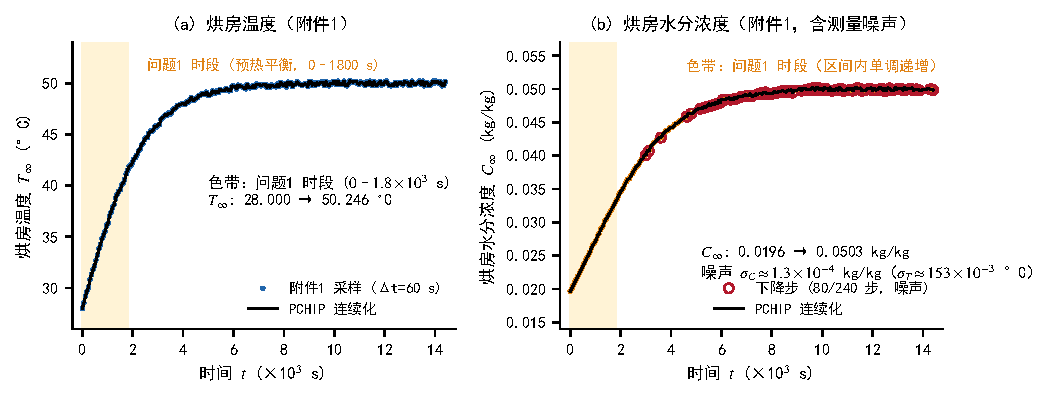
\includegraphics[width=0.86\textwidth]{figures/fig_q1_env.pdf}
    \caption{附件~1 给出的烘房环境激励。色带为问题一使用的预热平衡时段
    ($0\sim1800\,\mathrm{s}$)；(b) 中圆圈标出水分浓度序列出现下降的采样步
    （$80/240$ 步），表明数据含测量噪声，而问题一时段内序列单调。}
    \label{fig:env}
\end{figure}

\section{模型的建立与求解}
\label{sec:model}

\subsection{问题一模型的建立与求解}

\subsubsection{建模思路}

因为问题给出的圆柱体的长度和半径相差太多，
所以在对药材进行建模时，
可以将圆柱体视为一个无限长的圆柱体，
水分的扩散和温度变化只需要考虑径向的变化。
将模型简化代入Fourier导热定律的能量守恒形式以及Fick扩散方程得到其一维形式后，
可以知道其中的热扩散系数$\alpha$ 和水分扩散系数$D(C)$都时含水率$C$的函数，而$C$又是时间和空间的函数，
但是由于题目要求和问题假设，可以将两个方程进行解耦
所以求解过程中将两个方程独立求解。

\subsubsection{一维Fourier导热定律的能量守恒形式}

根据问题假设以及题目条件，
由于在预热阶段温度缓慢上升减少了自然对流和热冲击效应，
故我们只考虑导热过程中的能量守恒而不考虑动量守恒。
Fourier导热定律的能量守恒形式为:
\begin{equation}
\rho c \frac{\partial T}{\partial t}=\nabla \cdot (k\nabla T)+\dot\Phi_v
\end{equation}
其中$\alpha=\frac{k}{\rho c}$为热扩散系数，$k$为热传导系数，
又因为轴径比过大且不考虑体积内热源，
所以可以将其简化为在圆柱坐标系下的一维Fourier导热定律的能量守恒形式，
即
\begin{equation}
\frac{\partial T}{\partial t}=\frac{\alpha}{r}\frac{\partial}{\partial r}(r\frac{\partial T}{\partial r})
\end{equation}
物理模型与边界条件如图~\ref{fig:model} 所示：热量自药材表面进入内部，表面以第三类边界
$hA_s\,(T_\infty-T)$ 与烘房换热，中心由对称性温度梯度为零。
\begin{figure}[htbp]
    \centering
    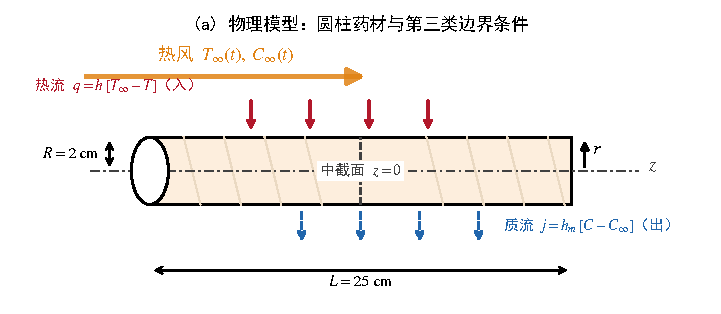
\includegraphics[width=0.72\textwidth]{figures/fig_q1_model.pdf}
    \caption{圆柱药材物理模型与第三类边界条件}
    \label{fig:model}
\end{figure}

\subsubsection{一维Fick扩散方程}

水分总是表面的先蒸发，而内部的水分蒸发是通过扩散现象扩散至表面进行蒸发，所以需要建立扩散方程。
圆柱坐标下的Fick第二定律为：
\begin{equation}
    \frac{\partial C}{\partial t}=D(C)\bigl[\frac{1}{r}\frac{\partial}{\partial r}(r\frac{\partial C}{\partial r})+\frac{1}{r^2}\frac{\partial^2 C}{\partial \phi^2}+\frac{\partial^2C}{\partial z^2}\bigr]
\end{equation}
由于在轴径比过大，所以将圆柱体视为无限长的圆柱体，那么就只需要考虑径向扩散，
原模型可以简化为
\begin{equation}
    \frac{\partial C}{\partial t}=\frac{1}{r}\frac{\partial}{\partial r}(rD(C)\frac{\partial C}{\partial r})
\end{equation}
水分扩散的物理图景如图~\ref{fig:fick} 所示：预热阶段内部含水率几乎保持初值
$C_0$，水分在浓度梯度驱动下向表面输运，并经对流传质边界蒸发进入烘房。
\begin{figure}[htbp]
    \centering
    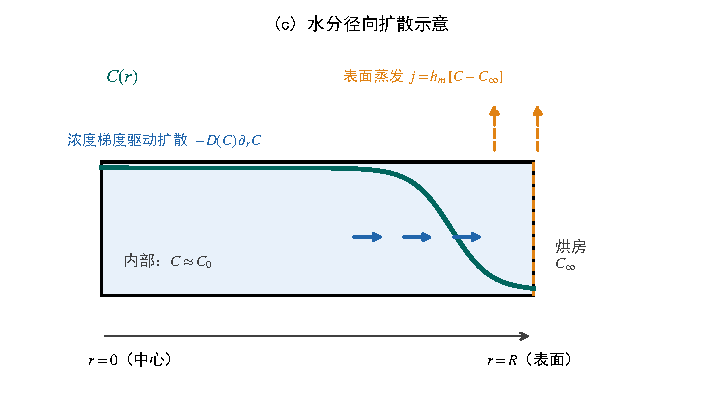
\includegraphics[width=0.72\textwidth]{figures/fig_q1_fick.pdf}
    \caption{水分扩散示意图：浓度梯度驱动水分向表面输运并蒸发}
    \label{fig:fick}
\end{figure}


\subsubsection{初始条件与边界条件}

方程（2）与（4）配以定解条件即构成完整的初边值问题。初始时刻药材温度与含水率
均匀；中心$r=0$处由轴对称性给出零梯度；表面$r=R$处与烘房通过对流换热、对流传质
耦合（第三类边界，见图~\ref{fig:model}），即
\begin{equation}
\left\{
\begin{aligned}
    &T(r,0)=28\,^\circ\mathrm{C},\qquad C(r,0)=2.55\,\mathrm{kg/kg}, &&\text{（初始条件）}\\[1pt]
    &\partial_r T\big|_{r=0}=\partial_r C\big|_{r=0}=0, &&\text{（中心对称）}\\[1pt]
    &-k\,\partial_r T\big|_{r=R}=h\,\bigl[T(R,t)-T_\infty(t)\bigr], &&\text{（表面换热）}\\[1pt]
    &-D\,\partial_r C\big|_{r=R}=h_m\,\bigl[C(R,t)-C_\infty(t)\bigr], &&\text{（表面传质）}
\end{aligned}
\right.
\end{equation}
其中对流换热系数$h=25\,\mathrm{W/(m^2\cdot K)}$、对流传质系数
$h_m=8\times10^{-7}\,\mathrm{m/s}$ 均按附录~2 给定；烘房环境$T_\infty(t)$、
$C_\infty(t)$ 由附件~1 数据经保形分段三次插值（PCHIP）连续化——PCHIP 在采样节点
处一阶连续、区间内保形单调，对附件~1 中$C_\infty$序列的测量噪声不会产生虚假极值，
其光滑性满足与隐式格式联立求解的要求。计算中温度以热力学温度 K 为状态变量，
输出时再折算回$^\circ$C。

\subsubsection{求解某一时刻下药材各个位置的温度}
\label{sec:tempsolve}

由于在一维Fourier导热定律的能量守恒形式中，热扩散系数$\alpha$为常数、与含水量无关，
方程对$T$线性；但边界条件随烘房环境变化，且题目要求四位小数的结果精度，
所以将方程中的微分形式离散，用数值方法逐层递推求解。总体思路是：空间上作守恒型
有限体积离散，时间上作全隐式差分，把偏微分方程化为每个时间步的一个三对角线性
方程组。求解分为以下三步。

\noindent\ding{228}\ \textbf{空间离散：节点式网格与控制体}

将半径$[0,R]$均分为$M$段，取节点$r_i=i\Delta r$（$i=0,1,\dots,M$，$\Delta r=R/M$），
$r=0$与$r=R$均为节点，使题目要求的输出位置$0,0.1,\dots,2.0\,\mathrm{cm}$恰好落在
节点上（图~\ref{fig:fvm}）。节点$i$的控制体为$[r_{i-1/2},r_{i+1/2}]$，其体积与
两个界面的面积（单位轴长）为
\begin{equation}
V_i=\pi\bigl(r_{i+1/2}^2-r_{i-1/2}^2\bigr),\qquad A_{i\pm1/2}=2\pi r_{i\pm1/2},
\end{equation}
对每个控制体作能量平衡（净流入热量$=$内能增量），得到半离散方程
\begin{equation}
\frac{dT_i}{dt}=\frac{\alpha}{\Delta r}\Bigl[f_i^{+}\bigl(T_{i+1}-T_i\bigr)
-f_i^{-}\bigl(T_i-T_{i-1}\bigr)\Bigr],
\qquad f_i^{\pm}=\frac{A_{i\pm1/2}}{V_i}=\frac{2i\pm1}{2i\,\Delta r}.
\end{equation}

\noindent \ding{228}\ \textbf{时间离散：全隐式Euler与三对角方程组}

时间导数取$\frac{dT_i}{dt}\approx\frac{T_i^{n+1}-T_i^n}{\Delta t}$，右端同样取
$n+1$时刻（全隐式），整理后每个内部节点给出三对角方程
\begin{equation}
a_iT_{i-1}^{n+1}+b_iT_i^{n+1}+c_iT_{i+1}^{n+1}=\frac{T_i^n}{\Delta t},
\end{equation}
其中
\begin{equation}
a_i=-\frac{\alpha(i-\tfrac12)}{i\Delta r^2},\qquad
b_i=\frac{1}{\Delta t}+\frac{2\alpha}{\Delta r^2},\qquad
c_i=-\frac{\alpha(i+\tfrac12)}{i\Delta r^2}.
\end{equation}
三系数行和$a_i+b_i+c_i=0$恒成立，保证离散能量守恒且解满足极值原理。两个边界行
单独处理：中心$r=0$由对称性用半控制体，得$b_0=1/\Delta t+4\alpha/\Delta r^2$、
$c_0=-4\alpha/\Delta r^2$；表面$r=R$为半控制体，外侧界面直接代入第三类边界的真实
热流$hA_s(T_\infty-T_M)$，得右端多出$g_hT_\infty^{n+1}$，其中
$g_h=A_sh/(\rho c_pV_M)$，$A_s=2\pi R$，$T_\infty^{n+1}$由附件~1的PCHIP插值取值
——烘房激励由此进入递推。

\noindent\ding{228}\ \textbf{追赶法逐层递推}

每个时间步的方程组是严格对角占优的三对角系统
（$b_i-(|a_i|+|c_i|)=1/\Delta t>0$），用追赶法以$O(M)$直接求解，以伪代码形式呈现如下：

\begin{center}
\begin{minipage}{0.92\textwidth}
\centering\small
\textbf{表~1\quad 温度场的数值求解伪代码 }\\[3pt]
\begin{tabular}{cp{0.80\textwidth}}
\toprule
温度场求解伪代码 \\
\midrule
1 & \textbf{输入}：网格数$M$、时间步长$\Delta t$、初值$T_i^0=28\,^\circ\mathrm{C}$；由附件~1的PCHIP插值得到$T_\infty(t)$ \\
2 & \textbf{for} $n=0,1,\dots,1800/\Delta t-1$：取$T_\infty^{n+1}$ \\
3 & \qquad 组装三对角系数$(a_i,b_i,c_i)$与右端$d_i=T_i^n/\Delta t$（表面行加$g_hT_\infty^{n+1}$） \\
4 & \qquad 追赶法求解得$T^{n+1}$ \\
5 & $n\leftarrow n+1$；若$t<1800\,\mathrm{s}$转入\textbf{Step 2}，否则\textbf{输出}$T(r_i,t)$，$t=1,2,\dots,1800\,\mathrm{s}$ \\
\bottomrule
\end{tabular}
\end{minipage}
\end{center}

算法中的系数$(a_i,b_i,c_i)$只依赖$\alpha$、网格与$\Delta t$，整个计算只组装一次，
每个时间步仅更新右端；全隐式Euler对任意步长无条件稳定，故$\Delta t$只由精度决定。

从初始温度场$T_0\equiv28\,^\circ\mathrm{C}$出发，按算法逐层推进至
$1800\,\mathrm{s}$，即可求得任意时刻药材各位置的温度。每步计算量为$O(M)$，生产
设置取$M=3200$、$\Delta t=2^{-8}\,\mathrm{s}$（$1\,\mathrm{s}$恰为第$256$步），
论文表~1、表~2与\texttt{result1.xlsx}即按此流程计算得到。水分浓度场
的求解与上述流程完全同构，只需把$\alpha$换成界面平均后的$D(C)$、把表面热流换成
对流传质项，此处不再赘述。

\begin{figure}[htbp]
    \centering
    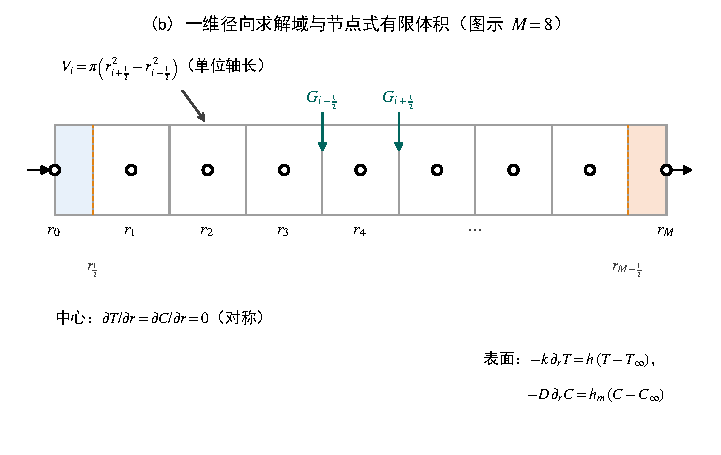
\includegraphics[width=0.72\textwidth]{figures/fig_q1_fvm.pdf}
    \caption{一维径向求解域与节点式有限体积网格（图示$M=8$）}
    \label{fig:fvm}
\end{figure}

\subsubsection{某时刻下药材各位置的温度结果呈现}

按\S\ref{sec:tempsolve} 的算法与生产设置（$M=3200$、$\Delta t=2^{-8}\,\mathrm{s}$）从
$T^0\equiv28\,^\circ\mathrm{C}$ 逐层推进至 $1800\,\mathrm{s}$，得到每隔 $1\,\mathrm{s}$、
每隔 $0.1\,\mathrm{cm}$ 的温度场，共 $1800\times21$ 个值。结果按题面要求以表~1 的格式
呈现，并配以时空演化可视化（图~\ref{fig:tempresults}）。

\noindent\ding{228}\ \textbf{表1：30分钟内药材的温度}

按题面表1的格式，给出 $100,300,600,900,1200,1500,1800\,\mathrm{s}$ 时刻、到药材中心
距离 $0,0.5,1,1.5,2\,\mathrm{cm}$ 处的温度，全部保留四位小数：

\begin{table}[htbp]
    \centering
    \caption{30 分钟内药材的温度（单位：$^\circ$C）}
    \label{tab:t1}
    \begin{tabular}{rccccc}
    \toprule
    时间/s & 0 cm & 0.5 cm & 1 cm & 1.5 cm & 2 cm \\
    \midrule
    100 & 28.0000 & 28.0003 & 28.0039 & 28.0319 & 28.1795 \\
    300 & 28.0406 & 28.0634 & 28.1513 & 28.3673 & 28.8486 \\
    600 & 28.4534 & 28.5361 & 28.8039 & 29.3156 & 30.1641 \\
    900 & 29.3243 & 29.4583 & 29.8758 & 30.6164 & 31.7295 \\
    1200 & 30.5429 & 30.7099 & 31.2225 & 32.1130 & 33.4295 \\
    1500 & 31.9960 & 32.1871 & 32.7667 & 33.7476 & 35.1211 \\
    1800 & 33.5758 & 33.7724 & 34.3642 & 35.3622 & 36.7858 \\
    \bottomrule
    \end{tabular}
\end{table}

\noindent\ding{228}\ \textbf{时空演化可视化}

图~\ref{fig:tempresults} 给出温度场的三种视图。(a) 时空热图直观展示热量自表面向
中心渗透的过程：等温线随时间由表面向内部推移，越靠近中心响应越滞后；(b) 径向剖面
显示径向梯度随时间增大——$t=100\,\mathrm{s}$ 时仅表面薄层升温，$t=1800\,\mathrm{s}$
时径向温差已达 $3.21\,^\circ\mathrm{C}$；(c) 演化曲线呈现三级滞后：
$T_\infty(1800\,\mathrm{s})=41.51\,^\circ\mathrm{C}$ 高于表面
$36.7858\,^\circ\mathrm{C}$（差 $4.7\,^\circ\mathrm{C}$），表面又高于中心
$33.5758\,^\circ\mathrm{C}$（差 $3.21\,^\circ\mathrm{C}$）。

\begin{figure}[htbp]
    \centering
    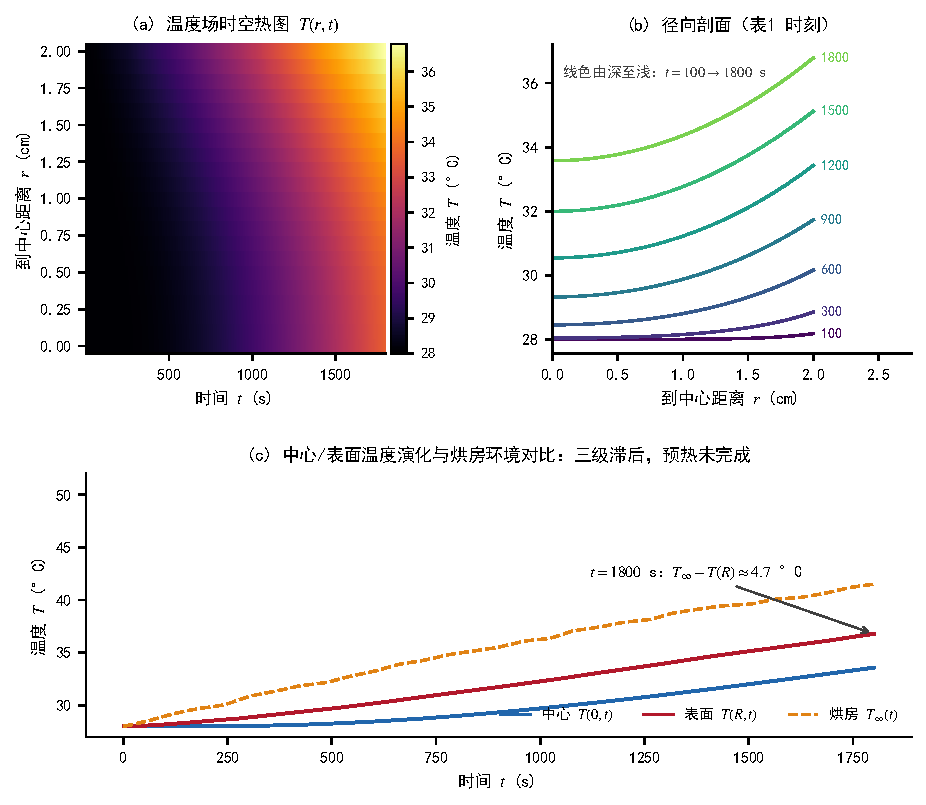
\includegraphics[width=0.96\textwidth]{figures/fig_q1_temp_results.pdf}
    \caption{问题一温度场结果。(a) 温度场时空热图；(b) 表1 时刻的径向剖面；
    (c) 中心/表面温度演化与烘房环境对比。}
    \label{fig:tempresults}
\end{figure}

\noindent\ding{228}\ \textbf{完整结果文件 result1.xlsx}

按附件~3 模板将完整结果写入 \texttt{result1.xlsx}``温度''工作表：A 列为时间
（$1,2,\dots,1800\,\mathrm{s}$），第 1 行为到药材中心的距离
（$0,0.1,\dots,2.0\,\mathrm{cm}$），共 $1800\times21$ 个值，全部保留四位小数；
``水分浓度''工作表结构相同（其求解与结果见后文）。

上述结果与问题分析的预判一致：热 Biot 数 $\mathrm{Bi}=1.389>0.1$ 使径向温差显著、
不可按集总参数处理；导热特征时间 $R^2/\alpha=2368.9\,\mathrm{s}$ 大于 $1800\,
\mathrm{s}$，故预热平衡阶段结束时热平衡尚未完成。数值上，本节结果与独立加密解的
偏差小于 $3.8\times10^{-6}\,\mathrm{K}$、与 Robin 圆柱解析级数解的偏差小于
$4.5\times10^{-6}\,\mathrm{K}$，远低于四位小数的分辨率（半 ulp $5\times10^{-5}$），
四位小数报告是安全的。

\subsubsection{求解某一时刻下药材各个位置的水分浓度}

水分方程的离散框架与温度场完全同构：同一节点式网格、同一全隐式 Euler、同一追赶法。
但有两点不同，需要专门处理：其一，扩散系数$D(C)$依赖未知量$C$本身，是非线性项；
其二，表面边界是对流传质而非热流。求解同样分为三步。

\noindent\ding{228}\ \textbf{界面扩散系数的守恒取法}

守恒型格式要求\textbf{同一条界面上的通量取单一的扩散系数}。若直接用节点值
$D(C_i)$ 充当节点$i$两侧界面的系数，则界面$r_{i+1/2}$从左侧控制体看是$D(C_i)$、
从右侧控制体看是$D(C_{i+1})$，两者不等，离散水量不再守恒：以全局水量收支
$\sum_iV_i\,(C_i^{n+1}-C_i^n)$ 对表面累计通量的闭合差为指标，节点值取法的残差达
表面总通量的$10.1\%$，且网格加密（$M=100,200,400$）时不减小
（$10.10\%,10.12\%,10.12\%$），属相容性错误。因此本文取相邻节点的算术平均
\begin{equation}
D_{i+1/2}=\frac{D(C_i)+D(C_{i+1})}{2},
\end{equation}
使同一条界面在两侧控制体中取值相同；此时全局水量收支残差降至$10^{-14}$量级
（机器精度），离散水量守恒。

\noindent\ding{228}\ \textbf{半隐式线性化与三对角方程组}

$D(C)$依赖未知量，严格处理需每步Newton迭代。考虑到问题一时段内$D$的变化幅度
有限（由$D(C_0)=4.9377\times10^{-9}$降至$D(1.51)=3.88\times10^{-9}\,
\mathrm{m^2/s}$，约$21\%$），本文将$D$用上一时刻的$C^n$计算（半隐式），
每步仍只解一个线性三对角系统：
\begin{equation}
a_i^CC_{i-1}^{n+1}+b_i^CC_i^{n+1}+c_i^CC_{i+1}^{n+1}=\frac{C_i^n}{\Delta t},
\end{equation}
系数与温度方程完全同构，只需把$\alpha$换成界面值$D_{i\pm1/2}$（$f_i^\pm$不变），
故严格对角占优依然成立。表面行的对流传质项$g_m=A_sh_m/V_M$不含$D$，右端多出
$g_mC_\infty^{n+1}$，$C_\infty^{n+1}$由附件~1的PCHIP插值取值。该半隐式近似的误差
用全非线性方法（线条法+BDF，$D$每步取当前值）校核：$\max|\Delta C|=
5.32\times10^{-6}\,\mathrm{kg/kg}$，远低于四位小数的分辨率。干燥后期
（问题二$\sim$四）$C$逼近$0.15\,\mathrm{kg/kg}$时$D$变化约$266$倍，届时改用
预测--校正或全隐式Newton迭代。

\noindent\ding{228}\ \textbf{追赶法逐层递推}

水分场的完整递推流程如算法~2所示，与算法~1在同一时间循环内先后执行。

\begin{center}
\begin{minipage}{0.92\textwidth}
\centering\small
\textbf{算法~2\quad 水分浓度场的数值求解流程（每个时间步）}\\[3pt]
\begin{tabular}{cp{0.80\textwidth}}
\toprule
Step & 操作 \\
\midrule
1 & \textbf{输入}：网格数$M$、时间步长$\Delta t$、初值$C_i^0=2.55\,\mathrm{kg/kg}$；由附件~1的PCHIP插值得到$C_\infty(t)$ \\
2 & \textbf{for} $n=0,1,\dots,1800/\Delta t-1$：取$C_\infty^{n+1}$ \\
3 & \qquad 由$C^n$计算界面扩散系数$D_{i+1/2}=\frac{1}{2}\bigl[D(C_i)+D(C_{i+1})\bigr]$ \\
4 & \qquad 组装三对角系数（$\alpha\to D_{i\pm1/2}$，表面行加$g_mC_\infty^{n+1}$）与右端$d_i=C_i^n/\Delta t$ \\
5 & \qquad 追赶法求解得$C^{n+1}$ \\
6 & $n\leftarrow n+1$；若$t<1800\,\mathrm{s}$转入\textbf{Step 2}，否则\textbf{输出}$C(r_i,t)$，$t=1,2,\dots,1800\,\mathrm{s}$ \\
\bottomrule
\end{tabular}
\end{minipage}
\end{center}

从初始浓度场$C^0\equiv2.55\,\mathrm{kg/kg}$出发，按算法~2逐层推进至
$1800\,\mathrm{s}$，即得水分浓度场；界面平均格式保证全程离散水量守恒。

\subsubsection{某时刻下各位置的水分浓度结果呈现}

按算法~2与生产设置（$M=3200$、$\Delta t=2^{-8}\,\mathrm{s}$）推得水分浓度场，
按题面表2的格式呈现，并配以时空演化可视化（图~\ref{fig:moistresults}）。

\ding{228}\ \textbf{表2：30分钟内药材的水分浓度}

按题面表2的格式，给出与表1相同时刻、相同位置的水分浓度，全部保留四位小数：

\begin{table}[htbp]
    \centering
    \caption{30 分钟内药材的水分浓度（单位：kg/kg）}
    \label{tab:t2}
    \begin{tabular}{rccccc}
    \toprule
    时间/s & 0 cm & 0.5 cm & 1 cm & 1.5 cm & 2 cm \\
    \midrule
    100 & 2.5500 & 2.5500 & 2.5500 & 2.5500 & 2.2470 \\
    300 & 2.5500 & 2.5500 & 2.5500 & 2.5492 & 2.0508 \\
    600 & 2.5500 & 2.5500 & 2.5500 & 2.5353 & 1.8770 \\
    900 & 2.5500 & 2.5500 & 2.5497 & 2.5045 & 1.7547 \\
    1200 & 2.5500 & 2.5500 & 2.5482 & 2.4646 & 1.6586 \\
    1500 & 2.5500 & 2.5499 & 2.5445 & 2.4206 & 1.5787 \\
    1800 & 2.5500 & 2.5497 & 2.5383 & 2.3755 & 1.5102 \\
    \bottomrule
    \end{tabular}
\end{table}

\ding{228}\ \textbf{时空演化可视化}

图~\ref{fig:moistresults} 给出水分场的三种视图。(a) 时空热图与温度场形成鲜明
对照：全场几乎同为初值色，仅表面薄层随时间变深——水分只在表层变化；(b) 径向剖面
呈``干壳''形态：内部平坦、表层骤降，且$t=100\,\mathrm{s}$时表层即已明显脱水；
(c) 各层浓度曲线显示：中心含水率几乎不动，相对下降仅$3.01\times10^{-6}$，体积
平均含水率下降$10.1\%$，表面降至$1.5102\,\mathrm{kg/kg}$较初值下降$40.8\%$，
而$C_\infty(1800\,\mathrm{s})=0.0331\,\mathrm{kg/kg}$，$C(R)/C_\infty\approx45.7$
——表面远未与热风平衡，干燥驱动力依然充足。

\begin{figure}[htbp]
    \centering
    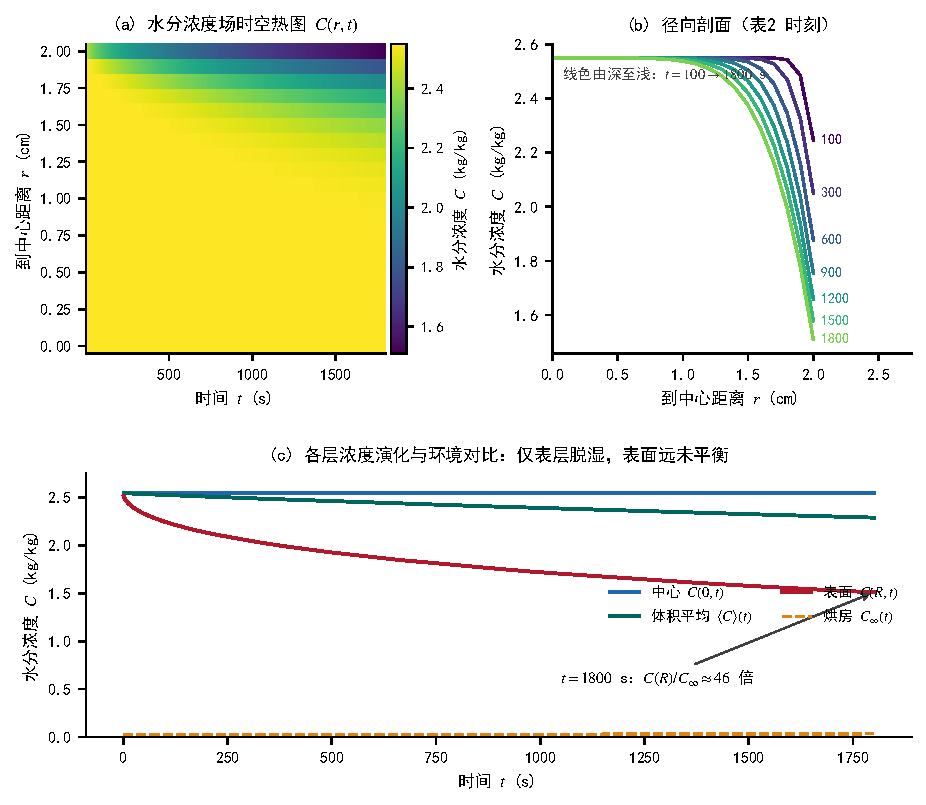
\includegraphics[width=0.96\textwidth]{figures/fig_q1_moist_results.pdf}
    \caption{问题一水分浓度场结果。(a) 水分浓度场时空热图；(b) 表2 时刻的径向剖面；
    (c) 各层浓度演化与烘房环境对比。}
    \label{fig:moistresults}
\end{figure}

上述形态由时间尺度分离决定：湿分扩散特征时间$R^2/D(C_0)=81010\,\mathrm{s}$远大于
$1800\,\mathrm{s}$，约为导热特征时间的$34$倍，水分来不及扩散到中心。数值上，
半隐式$D$的偏差为$5.32\times10^{-6}\,\mathrm{kg/kg}$、与独立加密解的偏差小于
$1.2\times10^{-5}\,\mathrm{kg/kg}$，低于四位小数的分辨率，报告是安全的。此外，
$D(C)$随$C$下降而骤减，$C=0.15$处比初值小约$266$倍，干燥前沿的``干壳''将使
后期干燥显著减慢，这是问题三确定烘干时间时需要专门处理的时间尺度问题。

\subsection{问题二模型的建立与求解}
% TODO：附录3 变物性与 D(C,T) 双向耦合模型的建立、交替迭代求解，表3/表4 与 result2.xlsx

\subsection{问题三模型的建立与求解}
% TODO：以各处 C < 0.15 kg/kg 为终止条件的事件定位，表5 与 result3.xlsx

\subsection{问题四模型的建立与求解}
% TODO：xi=r/R(t) 动边界与附录4 物性，表6 与 result4.xlsx

\section{模型评价与推广}
% TODO：优点、缺点、改进与推广

%参考文献
\begin{thebibliography}{9}%宽度9
    \bibitem{hu2020}
    胡众欢, 杨明金, 杨卓然, 杨玲.
    \newblock 基于多物理场耦合的热风干燥模型及其验证\allowbreak[J].
    \newblock 西南大学学报(自然科学版), 2020, 42(2): 118--128.
    \bibitem{rani2020}
    Rani P, Tripathy P P.
    \newblock Modelling of moisture migration during convective drying of pineapple slice considering non-isotropic shrinkage and variable transport properties\allowbreak[J].
    \newblock Journal of Food Science and Technology, 2020, 57(10): 3748--3761.
    \bibitem{oliveira2003}
    Oliveira P C, Lima J L.
    \newblock Flux-Spline discretization scheme applied to drying in capillary porous media\allowbreak[J].
    \newblock Revista Brasileira de Engenharia Agr\'icola e Ambiental, 2003, 7(1): 135--140.
    \bibitem{solomon2021}
    Solomon A B, Fanta S W, Delele M A, et al.
    \newblock Modeling and simulation of heat and mass transfer in an Ethiopian fresh injera drying process\allowbreak[J].
    \newblock Heliyon, 2021, 7: e06201.
    \bibitem{brasiello2021}
    Brasiello A, Venditti C, Adrover A.
    \newblock Non-isothermal moving-boundary model for food drying\allowbreak[J].
    \newblock Chemical Engineering Transactions, 2021, 87: 193--198.
    \bibitem{amankwah2018}
    Amankwah E A, Dzisi K A, van Straten G, et al.
    \newblock Moisture dependent diffusion and shrinkage in yam during drying\allowbreak[J].
    \newblock International Journal of Food Engineering, 2018, 14(7/8).
    \bibitem{marques2023}
    Marques B C, Flick D, Tadini C C, et al.
    \newblock Modeling convective drying of food products: the case study of yacon (\textit{Smallanthus sonchifolius})\allowbreak[R].
    \newblock Research Square 预印本, 2023.
\end{thebibliography}

\newpage
%附录
\begin{appendices}

\section{附录：结果文件与源程序}
% TODO：附上 result1--result4.xlsx 的生成方式与 Q1--Q4 核心代码（src/ 目录）

\end{appendices}

\end{document}
